
%(BEGIN_QUESTION)
% Copyright 2010, Tony R. Kuphaldt, released under the Creative Commons Attribution License (v 1.0)
% This means you may do almost anything with this work of mine, so long as you give me proper credit

This valve control circuit has a problem.  No matter what the setting on the hand indicating controller (HIC), the valve remains fully open all the time:

$$\includegraphics[width=15.5cm]{i00258x01.eps}$$

The technician before you used a clamp-on (Hall effect) milliammeter to check loop current at terminal 34 (cable HV-45a conductor), measuring 5.71 mA.  The same clamp-on meter used at the (+) terminal of the I/P converter showed 0 mA.

Determine the diagnostic value of each of the following tests.  Assume only one fault in the system, including any single component or any single wire/cable/tube connecting components together.  If a proposed test could provide new information to help you identify the location and/or nature of the one fault, mark ``yes.''  Otherwise, if a proposed test would not reveal anything relevant to identifying the fault (already discernable from the measurements and symptoms given so far), mark ``no.''

% No blank lines allowed between lines of an \halign structure!
% I use comments (%) instead, so that TeX doesn't choke.

$$\vbox{\offinterlineskip
\halign{\strut
\vrule \quad\hfil # \ \hfil & 
\vrule \quad\hfil # \ \hfil & 
\vrule \quad\hfil # \ \hfil \vrule \cr
\noalign{\hrule}
%
% First row
{\bf Diagnostic test} & {\bf Yes} & {\bf No} \cr
%
\noalign{\hrule}
%
% Another row
Measure DC voltage between terminals 34 and 35 &  &  \cr
%
\noalign{\hrule}
%
% Another row
Measure DC voltage between terminals 12 and 13 &  &  \cr
%
\noalign{\hrule}
%
% Another row
Measure DC voltage between both terminals labeled 12 (same block) &  &  \cr
%
\noalign{\hrule}
%
% Another row
Measure DC voltage between I/P terminals &  &  \cr
%
\noalign{\hrule}
%
% Another row
Measure DC current at terminal 35 (cable HV-45a conductor) &  &  \cr
%
\noalign{\hrule}
%
% Another row
Measure DC current at terminal 12 (cable HV-45b conductor) &  &  \cr
%
\noalign{\hrule}
%
% Another row
Measure DC current at terminal 12 (cable HV-45c conductor) &  &  \cr
%
\noalign{\hrule}
%
% Another row
Check air supply to see that it is at least 20 PSI &  &  \cr
%
\noalign{\hrule}
%
% Another row
Remove tube from valve diaphragm to check for air pressure there &  &  \cr
%
\noalign{\hrule}
} % End of \halign 
}$$ % End of \vbox

\vskip 20pt \vbox{\hrule \hbox{\strut \vrule{} {\bf Suggestions for Socratic discussion} \vrule} \hrule}

\begin{itemize}
\item{} The different current measurements at the two locations is a clear indication of what {\it type} of problem this is.  Identify the problem type, and explain how we know this to be so.
\item{} Given that this valve is air-to-close, and the hand controller is configured to read in percent open, does the indication of 89.3\% match the measured current of 5.71 mA?  Why or why not?
\end{itemize}

\underbar{file i00258}
%(END_QUESTION)





%(BEGIN_ANSWER)

% No blank lines allowed between lines of an \halign structure!
% I use comments (%) instead, so that TeX doesn't choke.

$$\vbox{\offinterlineskip
\halign{\strut
\vrule \quad\hfil # \ \hfil & 
\vrule \quad\hfil # \ \hfil & 
\vrule \quad\hfil # \ \hfil \vrule \cr
\noalign{\hrule}
%
% First row
{\bf Diagnostic test} & {\bf Yes} & {\bf No} \cr
%
\noalign{\hrule}
%
% Another row
Measure DC voltage between terminals 34 and 35 &  & $\surd$ \cr
%
\noalign{\hrule}
%
% Another row
Measure DC voltage between terminals 12 and 13 &  & $\surd$ \cr
%
\noalign{\hrule}
%
% Another row
Measure DC voltage between both terminals labeled 12 (same block) &  & $\surd$ \cr
%
\noalign{\hrule}
%
% Another row
Measure DC voltage between I/P terminals &  & $\surd$ \cr
%
\noalign{\hrule}
%
% Another row
Measure DC current at terminal 35 (cable HV-45a conductor) &  & $\surd$ \cr
%
\noalign{\hrule}
%
% Another row
Measure DC current at terminal 12 (cable HV-45b conductor) & $\surd$ &  \cr
%
\noalign{\hrule}
%
% Another row
Measure DC current at terminal 12 (cable HV-45c conductor) & $\surd$ &  \cr
%
\noalign{\hrule}
%
% Another row
Check air supply to see that it is at least 20 PSI &  & $\surd$ \cr
%
\noalign{\hrule}
%
% Another row
Remove tube from valve diaphragm to check for air pressure there &  & $\surd$ \cr
%
\noalign{\hrule}
} % End of \halign 
}$$ % End of \vbox

%(END_ANSWER)





%(BEGIN_NOTES)

Based on the two current measurements, we may conclude that the fault is a {\it short circuit} somewhere between terminals 34/35 and the terminals of the I/P.




\vskip 20pt \vbox{\hrule \hbox{\strut \vrule{} {\bf Virtual Troubleshooting} \vrule} \hrule}

This question is a good candidate for a ``Virtual Troubleshooting'' exercise.  Presenting the diagram to students, you first imagine in your own mind a particular fault in the system.  Then, you present one or more symptoms of that fault (something noticeable by an operator or other user of the system).  Students then propose various diagnostic tests to perform on this system to identify the nature and location of the fault, as though they were technicians trying to troubleshoot the problem.  Your job is to tell them what the result(s) would be for each of the proposed diagnostic tests, documenting those results where all the students can see.

During and after the exercise, it is good to ask students follow-up questions such as:

\begin{itemize}
\item{} What does the result of the last diagnostic test tell you about the fault?
\item{} Suppose the results of the last diagnostic test were different.  What then would that result tell you about the fault?
\item{} Is the last diagnostic test the best one we could do?
\item{} What would be the ideal order of tests, to diagnose the problem in as few steps as possible?
\end{itemize}


%INDEX% Troubleshooting review: electric circuit diagnostic test usefulness

%(END_NOTES)


